
This section is based on the Notes of the MasterClass given in Angers, France (2024) by Mattia Cafasso and Sofia Tarricone.

Let us consider the symmetric group $S_N$ of the permutations of the finite set $\{1, 2, \cdots, N\}$.
\begin{definition}
	Let $\pi \in S_n$ be a permutation. Given $k$ integers
	\begin{equation}
		1 \leq i_1 \leq i_2 \leq \cdots \leq i_k \leq N
	\end{equation}
	we say that $\pi(i_1), \cdots, \pi(i_k)$ is an increasing sub-sequence of $\pi$ of length $k$ if $\pi$ preserves the order of the integers $i_j$, $j = 1, \cdots, k$, i.e.
	\begin{equation}
		\pi(i_1) < \pi(i_2) < \cdots < \pi(i_k).
	\end{equation}
\end{definition}
We denote $l_N(\pi)$ the maximal length of all the increasing sub-sequences of $\pi$.

\begin{ex}
	Let $\pi = 54172386$. Then (by direct inpection), $l_N(\pi) = 4$. The maximal length sequences are $(1, 2, 3, 6)$ and $(1, 2, 3, 8)$.
\end{ex}

Some history on the problem can be enunciated as

\begin{enumerate}
	\item Stanislaw Ulam, in an article published in 1961, discussed the idea of using Monte Carlo approaches to study the asymptotic behavior of $\E[l_N]$, when $N \rightarrow \infty$. Based on his simulations, Ulam conjectured that it exists a constant $c$ such that $$\lim_{N \rightarrow \infty} \frac{\E[l_N]}{\sqrt{N}} = c.$$ The term Ulam's problem, originally, referred to the proof of this conjecture and the identification of the constant $c$. 
	\item Hammersley, in 1972, introduced a Poissonized version of this problem and proved that the constant $c$ exists. 
	\item In 1977, Logan and Shepp and, independently, Vershik and Kherov showed that $c = 2$. 
	\item Odlyzko and Rains, in the $90$'s, performed analytical simulations indicating that 
	\[
	\lim_{N \rightarrow \infty} \frac{\Var[l_N]}{N^{\frac{1}{3}}} = c_0 \equiv 0,819\cdots
	\]
	and also that
	\[
	\lim_{N \rightarrow \infty} \frac{\E[l_N] - 2\sqrt{N}}{N^{\frac{1}{6}}} = c_1 \equiv -1.748\cdots
	\]
\end{enumerate}

Finally, Ulam's problem was solved by Baik, Deift and Johansson in $1999$, who studied the convergence in distribution of the re-scaled variable 
\begin{equation}
	\chi_N \deff \frac{l_N - 2\sqrt{N}}{N^{\frac{1}{6}}}
\end{equation}
given by
\begin{thm}
	(Baik-Deift-Johansson, $1999$). Let $\chi$ be a random variable with distribution function $F_{GUE}(x)$. Then $\chi_N$, defined as before, converges in distribution to $\chi$: 
	\begin{equation}
		\lim_{N \rightarrow \infty} \p\left\{ \frac{l_N - 2\sqrt{N}}{N^{\frac{1}{6}}} \leq x\right\} \rightarrow F_{(2)}(x)
	\end{equation}
	we have, moreover, convergence of moments
	\begin{equation}
		\lim_{N \rightarrow \infty} \E[\chi_N^m] = \E[\chi^m], \ \forall m \geq 1.
	\end{equation}
\end{thm}

To study, there is a nice representation of the permutated sequences that is worth exploring.


\subsection{Young's Diagram - and Tableaus}

Consider the following process. Start with a deck of $N$ well shuffled cards (with uniform measure) - numbered $1, 2, \cdots, N$ for convenience. Now place the first card of the shuffled deck on the table. The second card will be placed on top of the first, if it is labeled with a smaller number, and on its side if it is labeled with a larger number. Now, if the third card is smaller than the two cards, it is again placed on top of both cards. If it is in-between it is placed on the side of the second card. If it is bigger than both, it is placed on the side of the first card. The fourth card follows the same process. This gives rise to what we call a \textit{Young's Diagram}.

\begin{definition}
	A partition $\lambda = (\lambda_1, \cdots, \lambda_r)$ of $N$ is a set of positive integers such that $\lambda_1 \geq \lambda_2 \geq  \cdots \geq \lambda_r$ and $|\lambda| \deff \sum_i \lambda_i = N$. We call $|\lambda|$ the size of the partition, and $r$ its length. We will sometimes write $\lambda \vdash N$ to indicate that $\lambda$ has size $N$. 
\end{definition}

A convenient graphic representation of integer partitions is given by Young diagrams, which are constructing stacking r rows of boxes, each of length $\lambda_i$, in decreasing order. For instance, the partition $(5, 5, 3, 3, 2, 1, 1) \vdash 20$ corresponds to the Young diagram below: 
\begin{figure}[h!]
	\centering
	\ydiagram{5,5,3,3,2,1,1}
	\caption{Young Diagram}
\end{figure}
The set of Young diagrams of size $N$ will be denoted $YN$, and the set of all Young diagrams $Y$. From now on, we will implicitly identify a partition and the corresponding Young diagram. 

\begin{definition}
	A Young tableau of size $N$ is a Young diagram $(\lambda_1, \cdots, \lambda_r) \vdash N$ together with a bijection between its boxes and the integers $\{1, \cdots , N\}$. A standard Young tableau is a Young tableau whose integers increase along the lines and the columns. We will denote with $SYT_N$ the set of standard Young tableau of size $N$. The Young diagram of a given Young tableau $P$, denoted $\sh(P)$, is called the shape of the tableau. 
\end{definition}

\begin{ex}
	The two Young tableaux below are of shape $(5, 5, 4, 2, 2, 1) \vdash 19$, the first one is standard and the second one is not. 
	\begin{figure}[h!]
		\centering
		\subfigure{
			\begin{ytableau}
				1 & 3 & 4 & 8 & 10 \\
				2 & 5 & 9 & 13 & 14 \\
				6 & 11 & 12 & 16 \\
				7 & 15 \\
				17 & 18 \\
				19 \\
			\end{ytableau}
		}
		\subfigure{
			\begin{ytableau}
				5 & 3 & 4 & 8 & 10 \\
				2 & 1 & 12 & 13 & 14 \\
				6 & 11 & 9 & 16 \\
				15 & 7 \\
				17 & 18 \\
				19 \\
			\end{ytableau}
		}
		\caption{Young Tableau}
	\end{figure}
\end{ex}
\begin{thm}
	If we define 
	\begin{equation}
		F_\lambda \deff \{P \in SYT_N \ : \ \sh(P) = \lambda \}
	\end{equation}	
	we have the following (amazing) identity
	\begin{equation}
		\sum_{\lambda \vdash N} F_\lambda^2 = N!
	\end{equation}
	derived using the so called Robinson-Schensted correspondence between Young's Tableau and permutations,
	\begin{equation}
		RS \ : \ S_N\rightarrow \{(P, Q) \in SYT_N \times SYT_N \ : \ \sh(P) = \sh(Q) \}
	\end{equation}
\end{thm}

The interesting part we want to discuss is when we actually change the convention a little for the Young Tableau. Namely, geometrically, we will rotate the diagram forty five degrees and centralize the bottom corner to be at the origin of a Real line. Now, we associate the $YT$ with the following set of numbers: If we have the $YT - (\lambda_1, \cdots, \lambda_n)$, then the set is given by 
\begin{equation}
	S(YT) = \left\{ \frac{\lambda_1 - 1}{2}, \frac{\lambda_2 - 3}{2}, \frac{\lambda_3 - 5}{2}, \cdots \right\}
\end{equation}
as depicted in the figure.
\begin{figure}[h!]
	\centering
	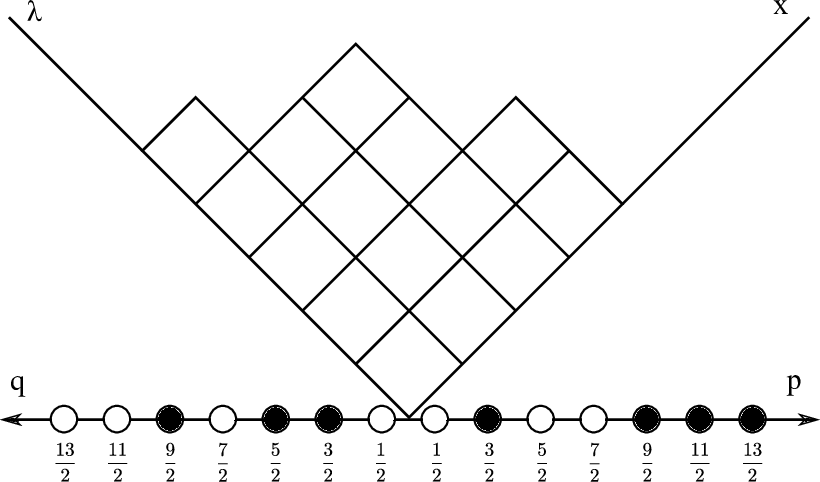
\includegraphics{./Assets/YoungTableauRotated.png}
\end{figure}
When we take the size of the $YT$ to be going to infinity we have a limiting shape represented below - this shape is well described.
%\begin{figure}[h!]
%	\centering
%	\subfigure{
	%		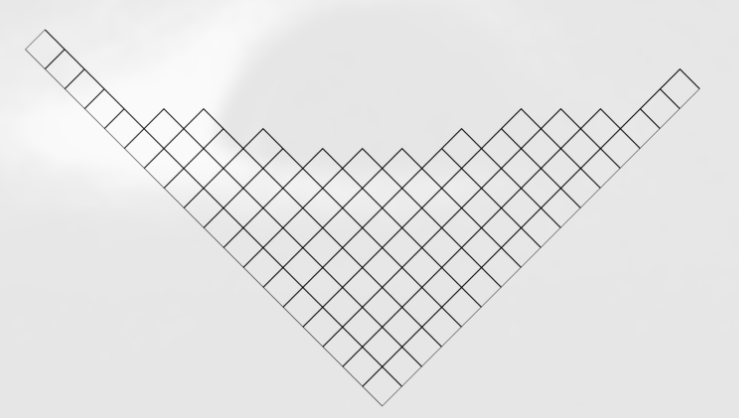
\includegraphics[width=0.45\linewidth]{./Assets/YTsmall.png}
	%	}
%	\subfigure{
	%		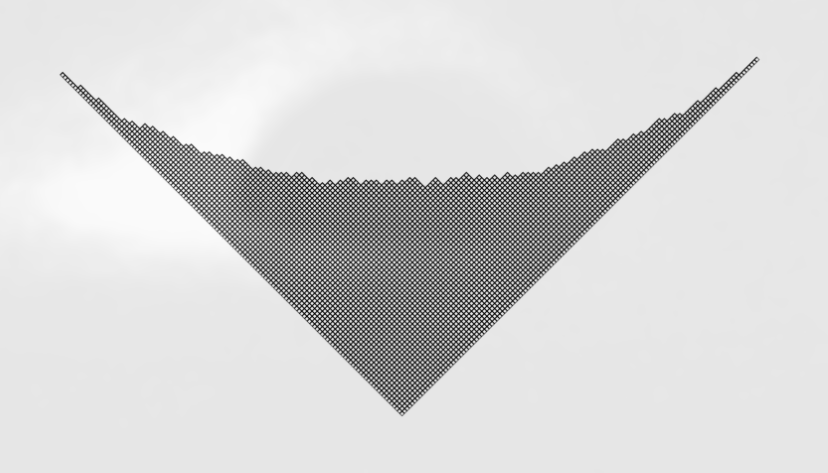
\includegraphics[width=0.45\linewidth]{./Assets/YTlarge.png}
	%	}
%\end{figure}
More interesting, we also have a limit distribution of associated points $S(YT)$. This is excitedly the same distribution of point we get for the eigenvalues of a matrix ensemble called Wigner Matrices.
